% mnras_template.tex 
%
% LaTeX template for creating an MNRAS paper
%
% v3.0 released 14 May 2015
% (version numbers match those of mnras.cls)
%
% Copyright (C) Royal Astronomical Society 2015
% Authors:
% Keith T. Smith (Royal Astronomical Society)

% Change log
%
% v3.0 May 2015
%    Renamed to match the new package name
%    Version number matches mnras.cls
%    A few minor tweaks to wording
% v1.0 September 2013
%    Beta testing only - never publicly released
%    First version: a simple (ish) template for creating an MNRAS paper

%%%%%%%%%%%%%%%%%%%%%%%%%%%%%%%%%%%%%%%%%%%%%%%%%%
% Basic setup. Most papers should leave these options alone.
\documentclass[fleqn,usenatbib]{mnras}

% MNRAS is set in Times font. If you don't have this installed (most LaTeX
% installations will be fine) or prefer the old Computer Modern fonts, comment
% out the following line
\usepackage{newtxtext,newtxmath}
% Depending on your LaTeX fonts installation, you might get better results with one of these:
%\usepackage{mathptmx}
%\usepackage{txfonts}

% Use vector fonts, so it zooms properly in on-screen viewing software
% Don't change these lines unless you know what you are doing
\usepackage[T1]{fontenc}
\usepackage{ae,aecompl}
\usepackage{color}
\newcommand\khb[1]{{\color{blue}#1}}
\newcommand\edits[1]{{\color{red}#1}}
\newcommand\aab[1]{{\color{green}#1}}

%%%%% AUTHORS - PLACE YOUR OWN PACKAGES HERE %%%%%

% Only include extra packages if you really need them. Common packages are:
\usepackage{graphicx}	% Including figure files
\usepackage{amsmath}	% Advanced maths commands
\usepackage{amssymb}	% Extra maths symbols
\usepackage{textgreek}
\usepackage{enumitem}
%%%%%%%%%%%%%%%%%%%%%%%%%%%%%%%%%%%%%%%%%%%%%%%%%%

%%%%% AUTHORS - PLACE YOUR OWN COMMANDS HERE %%%%%

% Please keep new commands to a minimum, and use \newcommand not \def to avoid
% overwriting existing commands. Example:
%\newcommand{\pcm}{\,cm$^{-2}$}	% per cm-squared

%%%%%%%%%%%%%%%%%%%%%%%%%%%%%%%%%%%%%%%%%%%%%%%%%%

%%%%%%%%%%%%%%%%%%% TITLE PAGE %%%%%%%%%%%%%%%%%%%

% Title of the paper, and the short title which is used in the headers.
% Keep the title short and informative.
\title[Abbie=Smart Person]{Serious Titles are Boring: predicting the future of dark matter halos is fun.}

% The list of authors, and the short list which is used in the headers.
% If you need two or more lines of authors, add an extra line using \newauthor
\author[Very Smart]{
Genius 1,$^{1}$\thanks{E-mail: mn@ras.org.uk (KTS)}
Genius 2,$^{2}$
and Genius 3$^{2,3}$
\\
% List of institutions
$^{1}$Royal Astronomical Society, Burlington House, Piccadilly, London W1J 0BQ, UK\\
$^{2}$Department, Institution, Street Address, City Postal Code, Country\\
$^{3}$Another Department, Different Institution, Street Address, City Postal Code, Country
}

% These dates will be filled out by the publisher
\date{Accepted XXX. Received YYY; in original form ZZZ}

% Enter the current year, for the copyright statements etc.
\pubyear{2018}


% Don't change these lines
\begin{document}
\label{firstpage}
\pagerange{\pageref{firstpage}--\pageref{lastpage}}
\maketitle

% Abstract of the paper
\begin{abstract}
\khb{The evolution of a dark matter halo in a dark matter only simulation is governed purely by Newtonian gravity, making a clean testbed to determine what halo properties drive its fate. Using machine learning, we predict the survival, mass loss, final position, and merging time of subhalos within a cosmological N-body simulation,
focusing on what instantaneous features of the halo, interaction, and environment matter most.}


%using the ability of these models to accurately make predictions as a proxy for the stochasticity of the underlying subhalo evolution.

Survival is well predicted, with 96.5\% accuracy, given only 3 parameters from the initial interaction. However, the mass loss, final location, and merging times are much more stochastic processes, requiring the definition of accuracy to allow for larger errors in prediction to reach similar accuracy percentages \khb{huh? rephrase after the comma} The scale factor, orbital eccentricity, relative velocity, and the masses of the host and subhalo are the only relevant parameters for determining subhalo evolution. In general, subhalos that enter their hosts at a mid-range of initial scale factor (typically a = .6-.8) are most challenging to make predictions for, across all of our final outcomes. More circular subhalo orbits are also easier to predict, except for in the case of predicting disruption, where the opposite appears to be true. We conclude that the detailed evolution of individual subhalos within N-body simulations is quite stochastic, with implications... \khb{I'd prefer redshift to scale factor, because I think more people use z than a}
\end{abstract}

% Select between one and six entries from the list of approved keywords.
% Don't make up new ones.
\begin{keywords}
me -- genius -- smart
\end{keywords}

%%%%%%%%%%%%%%%%%%%%%%%%%%%%%%%%%%%%%%%%%%%%%%%%%%

%%%%%%%%%%%%%%%%% BODY OF PAPER %%%%%%%%%%%%%%%%%%

\section{Introduction}

\khb{looking at the Annual Reviews of Astronomy and Astrophysics can help here -- adding a few to get you started!, but this is definitely not complete}

According to the standard \LambdaCDM model of cosmology, dark matter structures in the universe form hierarchically through series of mergers, with larger halos continuously growing through the accretion of smaller subhalos. Once independent halos themselves, these subhalos sink to the center of their "host" halos, losing mass along their orbits due to tidal effects and dynamical friction. However, as has been shown by modern cosmological N-body simulations (CITE, CITE, CITE), a significant number of such subhalos retain some of their mass, remaining as substructures within their hosts today. The study of these substructures has been fundamental to our understanding of many areas of astrophysics, from large-scale structure (CITE, CITE) to the formation and evolution of galaxies (CITE, CITE), 
\khb{https://www.annualreviews.org/doi/abs/10.1146/annurev-astro-081817-051756, https://www.annualreviews.org/doi/abs/10.1146/annurev-astro-081913-040019}
which relies on both accurate subhalo populations and evolution within these cosmological simulations (CITE, CITE).

\khb{https://www.annualreviews.org/doi/abs/10.1146/annurev-astro-091916-055313?intcmp=trendmd}

\khb{looking at the Annual Reviews of Astronomy and Astrophysics can help here -- adding a few to get you started}



Galaxy formation and evolution is commonly studied through modeling the evolution of the subhalos that these galaxies inhabit, with tools such as semi-analytic models (CITE, CITE). 
\khb{https://www.annualreviews.org/doi/abs/10.1146/annurev-astro-082812-140951?intcmp=trendmd}
These techniques typically rely on merger trees constructed from N-body simulations, along with analytic treatments of the physical processes that cause their evolution (CITE, CITE, CITE). These semi-analytic models often perform quite well, reproducing the statistical properties of subhalo populations (CITE, CITE, CITE). Other works have focused on reproducing specific properties of subhalos, such as disruption rates (CITE, CITE, CITE), mass loss histories (CITE, CITE, CITE), spatial distributions within host halos (CITE, CITE, CITE), and merging timescales (CITE, CITE, CITE). 

Although much work has been done to better model these processes and create prescriptions for subhalo evolution, the validity (\textit{doesn't seem like the right word}) of tuning models to the evolution within N-body simulations has remained relatively unexplored. N-body simulations produce consistent subhalo mass functions that have been shown to be converged down to small masses (CITE, CITE, CITE). However, it has not been explored in detail whether the evolution of an individual subhalo within these simulations is a truly deterministic process. These analytic models for subhalo evolution often rely on some set of parameters about the subhalo and host halo at the beginning of an interaction (CITE, CITE, CITE, CITE) to predict the final evolution of such subhalo. However, it may be that subhalo evolution within N-body simulations is a stochastic process, and interactions with similar properties do not necessarily behave in similar ways.

In this work, we use a merger tree generated from the dark matter only simulation VISHNU (CITE?) in order to determine the evolution and fate of subhalos, quantified by the aforementioned final quantities (i.e survival/disruption, mass loss, final location within host halo, merging timescale) using machine learning. We model these final conditions from initial conditions at the time of a subhalo entering its host. Using physically-motivated parameters from the time of the subhalos entry, we use machine learning to predict these final quantities of the subhalo, in the hopes of investigating to what degree subhalo fate is motivated by these parameters and to what degree the interaction is stochastic and cannot be predicted. If the mass loss from a subhalo is deterministic, a machine learning algorithm should be able to map subhalo fate to initial conditions. On the other hand, if there is a level of stochasticity in subhalo fate, whether from physics or from the simulation, there will remain large prediction errors, even when using a complete set of parameters. \textit{This feels very weirdly worded and/or not really concise. Need to revisit.}

Machine learning has emerged as a powerful tool in astrophysics in a variety of fields, such as gravitational wave data analysis, exoplanet detection, galaxy morphological classification, one more. (CITE, CITE, CITE). The ability of machine learning models to approximate any function using a large set of parameters provides a useful means of revealing complicated correlations when a direct analytic function cannot be found. Notably, \citet{Nadler2017} recently used machine learning to predict the survival or disruption of subhalos in a hydrodynamic simulation, using the initial conditions of their counterparts in a dark matter only simulation. They were quite successful, accurately predicting the results of 85\% of their subhalo population. Works like this are encouraging that machine learning can be used to fit these complicated interactions. \edits{However, in this work, although we only use a dark matter only simulation, we also hope to take our predictions a step further by also predicting the mass loss, final spatial position, and merging time of these subhalos.}

\texit{Not positive about this being here or in the section where I talk about the parameters we have? And how much to go through individual papers or just list off like: these are the most common ones for merge time: list, list, list, list (CITE, CITE, CITE, CITE) type deal. So for now, this is just an unfinished paragraph.}
As mentioned above, many works have already attempted to analytically model these subhalo evolution processes with much success. As such, we have selected similar or the same initial parameters that have been found to be important for subhalo evolution to use in our model. For subhalo survival, ....

In Section \ref{sec:simulation}, we describe the simulation and data that was used, as well as the methods to properly reduce the data into the desired sample. In Section \ref{sec:ML Methods}, we cover the machine learning methods used to create our predictive models. In Section \ref{sec:feature selection}, we discuss the feature selection methods used to reduce the number of parameters needed to make predictions. In Section \ref{sec:Results}, we share the results of our models for predicting each of our outcomes, including their performance and which parameters were needed as inputs to the model. Finally, in Section \ref{sec:Conclusion} we discuss implications of the results for both observation and theory.

\section{Description of the Data}
\label{sec:simulation}
\begin{figure}
	% To include a figure from a file named example.*
	% Allowable file formats are eps or ps if compiling using latex
	% or pdf, png, jpg if compiling using pdflatex
	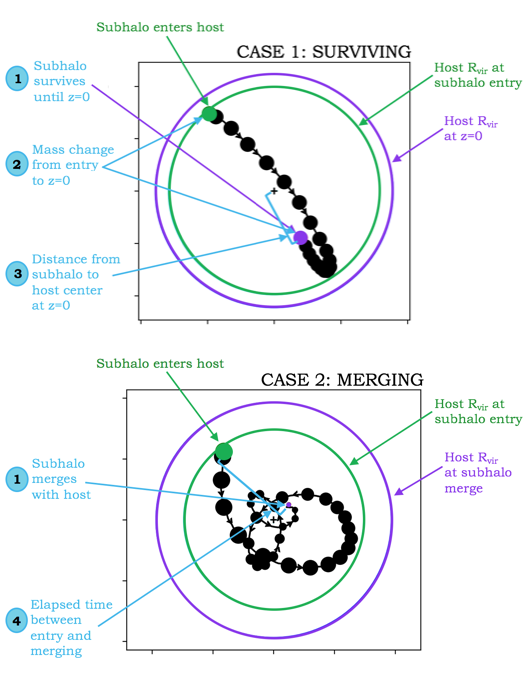
\includegraphics[width=\columnwidth]{Figures/explanatory_figures}
	\vspace{-15pt}
    \caption{An example of a surviving (top) and merging (bottom) interaction between a subhalo and host halo. The orbit of these two subhalos are shown within the radius of their respective host halos, shown by the larger, unfilled circles. Point size corresponds to subhalo mass along the orbit, plotted at each eighth timestep. The green point and circle show initial quantities, at the timestep right before the subhalo enters its host. The purple point and circle show final quantities, at either the timestep right before the subhalo dissolves in the merging case, or at the final timestep in the simulation in the surviving case. Predicted quantities (light blue) are labeled and numbered in the order they will be presented throughout the paper.}
    \label{fig:explanatory_figures}
\end{figure}

	Our analysis makes use of VISHNU, a cosmological N-body simulation with 1000 snapshots for exquisite time resolution; no snapshot is separated by more than X years. VISHNU contains 1680\textsuperscript{3} particles in a volume of 130h\textsuperscript{-1} cMpc and uses WMAP-1 cosmology (\citet{Spergel2003}; $\Omega$\textsubscript{m} = 0.25, $\Omega$\textsubscript{$\Lambda$} = 0.75, $\Omega$\textsubscript{b} = 0.04, $\sigma$\textsubscript{8} = 0.8, \textit{n\textsubscript{s}} = 1.0, \textit{h} = 0.7). Each dark matter particle has mass \textit{m\textsubscript{p}} = 3.215 $\times$ 10\textsuperscript{7}h\textsuperscript{-1} M\textsubscript{\(\odot\)}, and the force resolution is X parsecs. The ROCKSTAR halo finder was used to identify halos and subhalos, and merger trees were constructed with Consistent-Trees (\citet{Behroozi2013}).
\par
    Starting with halos at \textit{z}=0, we use the merger trees to identify the most massive progenitors of all host halos within the simulation, and track the subhalos within. These subhalos are allowed to have further substructure inside of them but cannot, at any point during their infall, become sub-substructure themselves. To help mitigate resolution uncertainties, we select only subhalos with a minimum of 1000 particles (total mass 3.215 $\times$ 10\textsuperscript{10}h\textsuperscript{-1} M\textsubscript{\(\odot\)}) at their time of accretion. We define the accretion time as the last timestep before a subhalo enters its host. 
    %As such, at the initial time of accretion, the will-be subhalos are still host halos themselves. Once the subhalo has entered its host, however, it cannot leave again (so, a flyby interaction would not be considered on its first pass but will be considered on a later pass if it falls back into and remains inside the host). 
    Once it has been accreted, the subhalo must have one of two fates: merge with the host, or remain a bound, identified subhalo within that host until today. We define the point of merging as the point right before dissolution of the subhalo, the last timestep in the simulation where it is identified as its own entity. Following uncertainties in subhalo mass loss shown by \citep{VandenBosch2018}, once a subhalo has lost more than 90\% of its mass, we also consider it to be merged. This cut changes the fates of only a small number of our subhalos, \edits{around 5\%}, but ensures a more consistent definition of merging that is less sensitive to resolution errors. \edits{Counts before/after 1000 particle cut, and before/after this 90\% loss cut is made}.
\par    
    Figure \ref{fig:explanatory_figures} shows examples of the orbits of the two types of interactions that we consider. In the top panel, we show an example of a surviving interaction, where the subhalo orbits for some time, losing mass but not dissolving before z=0. In the bottom panel, we show an example of a merging interaction, where the subhalo orbits and loses mass until reaching the center of the host and dissolving at some time before z=0. The four quantities that we will predict are shown in blue and numbered by the order that they will be presented in Section \ref{sec:Results}. We predict the survival of both the surviving and merging populations as one complete sample. When we predict the mass loss and final position quantities, we do so for only our surviving population. When we predict the merging time quantity, we do so for only the merging population. 
\par
    In addition to making cuts for resolution, some interactions were removed due to their unphysical behavior, likely as a result of errors in the merger tree generation or halo finding. \textbf{INSERT NUMBER} Subhalos were removed that gained more than 10 times their mass during infall. These subhalos were likely misidentified as they moved close to the center of the host, instead being assigned the mass of another subhalo or the host itself. \textbf{INSERT NUMBER} subhalos were removed because their initial mass was larger than that of its supposed host. \textbf{INSERT NUMBER} subhalos were removed because their positions were outside of the host virial radius. \edits{Actually, are these last two okay because I'm taking the timestep right before entry instead of right after?} \textbf{INSERT NUMBER} subhalos were removed because their time of merging was earlier than their time of entry?? \edits{Need to double check that those cases weren't errors in the writing out of the file or something, I think there were only like 5 so it's weird.} Altogether, we culled about 2\% of the total sample.
\par
	%Although we have attempted to correct for these errors, there remains the possibility that erroneous cases still exist within our sample. We have made a hard cut to remove halos that gain mass, but there may be still be cases where an identification of a halo was changed within our sample. Additionally, some orbits are known to look strange or have instantaneous mass loss or gain that can be harder to properly check for. \textit{Some discussion of the cases that could possibly still exist in the data due to difficulty in being able to filter them out/ find a general way to search for them? Lots of things that double/half mass in a step and then look semi-regular again. Should I mention that? Something that gives some estimation of how many cases might be like this? To ensure that it's not some large part of the sample and the reason we can't predict things. Mention that we removed about 2\% of the total number so even if you assume the same portion is wrong it shouldn't be the source of the stochasticity?}
\par

\begin{figure*}
	% To include a figure from a file named example.*
	% Allowable file formats are eps or ps if compiling using latex
	% or pdf, png, jpg if compiling using pdflatex
	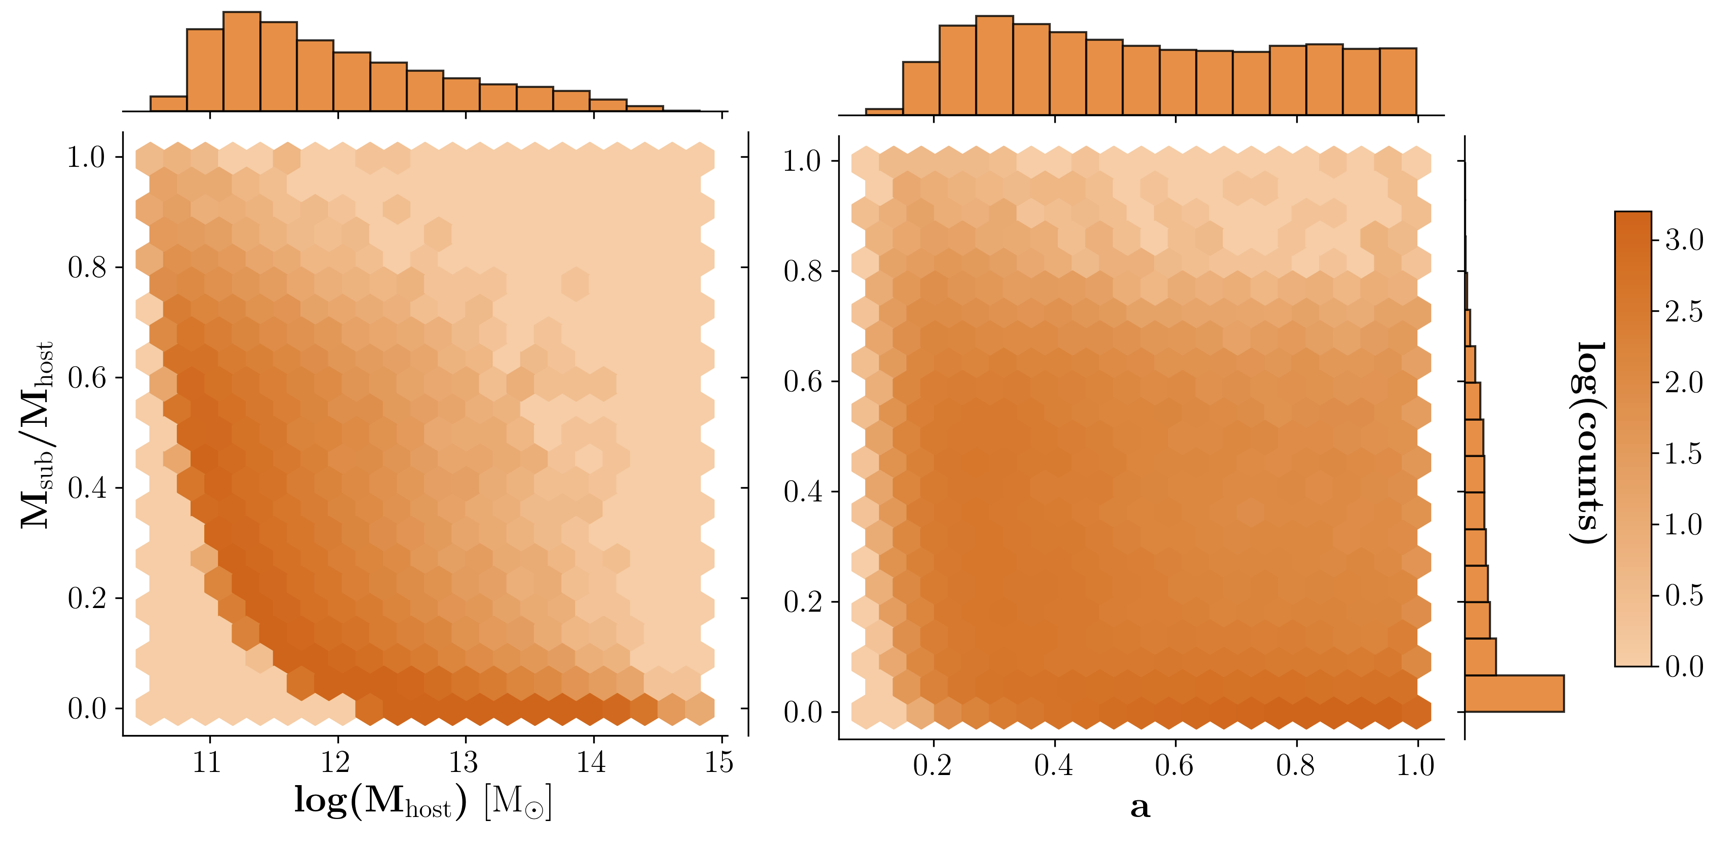
\includegraphics[width=\textwidth]{Figures/combined_distributions_logbin}
	\vspace{-20pt}
    \caption{Distributions of the merging interactions within our sample, in two different two-dimensional spaces. The left panel shows the distribution of interactions in the space of the host mass (x-axis) and the mass ratio (y-axis) of the interaction. The right panel shows the distribution of mergers in the space of the scale of initial entry of the subhalo (x-axis) and again, the mass ratio of the interaction on the y-axis. Within each hexagonal bin, the counts of interactions are shown, on a logarithm scale, by the colorbar. Histograms show the one-dimensional distribution of host masses (above the left panel), scale of entry (above the right panel) and mass ratios to the right of the right panel). Most interactions occur at lower mass ratios and for smaller host halos, but the spaces are still well-spanned over a range of interactions in both panels. The chosen cut of 1000 particles (M = 3.215 $\times$ 10\textsuperscript{10}h\textsuperscript{-1} M\textsubscript{\(\odot\)}) for subhalos upon entry is clearly shown in the left panel. Imposing this cut and requiring that host halos be larger than their subhalos means that, for very small host halos, the only subhalos within our dataset are those with masses more similar to their hosts. Additionally, it imposes that none of our host halos have masses below 3.215 $\times$ 10\textsuperscript{10}h\textsuperscript{-1} M\textsubscript{\(\odot\)} as well.}
    \label{fig:combined_distributions_logBin}
\end{figure*}

    Our resulting sample includes a total of \textbf{INSERT NUMBER} subhalo-halo interactions, with \textbf{INSERT NUMBER} of such being mergers and \textbf{INSERT NUMBER} being survivors. Distributions of this sample with respect to host masses, mass ratios, and the scale factor of the time of entry are shown in Fig.~\ref{fig:combined_distributions_logBin}. The most common interactions in our sample are mergers of unequal masses that occurred more recently. However, our sample also spans the space of more equal mass and higher redshift mergers, with hundreds of interactions shown in many of the bins in Fig.~\ref{fig:combined_distributions_logBin}. The effects of our chosen particle cut can also be clearly seen in Fig.~\ref{fig:combined_distributions_logBin}. Because subhalos must have 1000 particles at their time of entry, this results in a minimum initial mass of 3.215 $\times$ 10\textsuperscript{10}h\textsuperscript{-1} M\textsubscript{\(\odot\)} for both the subhalo and host halo, given that a host halo must also be at least as large as its subhalo. In the left panel of Fig.~\ref{fig:combined_distributions_logBin}, this results in an area of no data with low mass hosts and unequal masses, because most subhalos of low mass hosts are too low mass to be included in our sample. \edits{Say something about if these counts are typical/ what we expect to see/ agreement with other simulations?}
\par
    For both the host halo and subhalo at the timestep of infall, and at either the timestep right before merging or at z=0, we take several physically-motivated parameters to describe the interaction between the halos. A few additional parameters were not given explicitly from Consistent-Trees merger trees, but were calculated from some set of given parameters. We divide our final set of initial parameters, which were used as input parameters to the machine learning models to make predictions, into four main categories. Internal halo parameters are those that are properties of the individual halos themselves. These parameters do not depend on the other halo in the interaction, instead giving important information about the structure of the halos as individuals. Relative halo parameters describe properties of the halos that are dependent on either other halos within the simulation or the simulation itself. Orbital parameters provide information about the initial trajectory of the subhalo's infall path. Environmental parameters describe the influence of larger scale environment around the subhalo and its host. In total, this gives us 26 input parameters, with definitions:
    
\vskip 0.1in
    \noindent\textbf{Internal Halo Parameters:}
    \begin{itemize}[leftmargin=.4cm,topsep=0pt]
        \item \textbf{M\textsubscript{sub}}: M\textsubscript{200b} of the subhalo. This is defined using a spherical overdensity, including only those particles that were assigned to the subhalo. Because M\textsubscript{200b} is defined using the background mass density of the universe, this definition is not affected by pseudo-evolution.
        \item \textbf{M\textsubscript{host}}: M\textsubscript{200b} of the host halo. This is defined using a spherical overdensity, including all particles that are assigned as being part of the host halo. Therefore, this mass definition also includes the mass of all subhalos within the host.
        \item \textbf{R\textsubscript{sub}}: R\textsubscript{200b} of the subhalo.
        \item \textbf{R\textsubscript{host}}: R\textsubscript{200b} of the host halo.
        \item \textbf{c\textsubscript{sub}}: the concentration of the subhalo, defined as R\textsubscript{200b}/R\textsubscript{s}, where R\textsubscript{s} is the scale radius of the subhalo.
        \item \textbf{c\textsubscript{host}}: the concentration of the subhalo, defined as R\textsubscript{200b}/R\textsubscript{s}, where R\textsubscript{s} is the scale radius of the host halo.
        \item \textbf{\textlambda\textsubscript{sub}}: Bullock spin parameter of the subhalo, defined as in \citet{Bullock2001}.
        \item \textbf{\textlambda\textsubscript{host}}: Bullock spin parameter of the host halo, defined as in \citet{Bullock2001}.
        \item \textbf{T\textsubscript{sub}}: the triaxiality parameter of the subhalo. Calculated from the definition given in \citet{Franx1991}:
        \begin{equation}
            T = \frac{1 - (b/a)^2}{1 - (c/a)^2}
        \end{equation}
        where b/a is the minor/major axis ratio and c/a is the intermediate/major axis ratio.
        \item \textbf{T\textsubscript{host}}:  the triaxiality parameter of the host halo, calculated as above.
    \end{itemize}
\vskip 0.1in
    \noindent\textbf{Relative Halo Parameters:}
    \begin{itemize} [leftmargin=.4cm,topsep=0pt]
        \item \textbf{a}: the scale factor of the universe.
        \item \textbf{M\textsubscript{ratio}}: the ratio of subhalo to host halo masses.
         \item \textbf{max(M\textsubscript{subs,sub})}: M\textsubscript{200b} of the most massive sub-subhalo within the subhalo. 0 if subhalo has no sub-substrucutre. 
        \item \textbf{max(M\textsubscript{subs,host})}: M\textsubscript{200b} of the most massive subhalo already within the host halo at the time of the selected subhalo's entry. Does not include the selected subhalo. 0 if no other subhalos are present.
        \item \textbf{N\textsubscript{subs,sub}}: the total number of sub-subhalos within the subhalo.
        \item \textbf{N\textsubscript{subs,host}}:  the total number of subhalos within the host halo. Does not include the selected subhalo.
    \end{itemize}
\vskip 0.1in
    \noindent\textbf{Orbital Parameters:}
    \begin{itemize} [leftmargin=.4cm,topsep=0pt]
        \item \textbf{d\textsubscript{rel}}: relative absolute distance between the centers of the subhalo and host halo.
        \item \textbf{v\textsubscript{rel}}: relative total velocity between subhalo and host halo, calculated in the reference frame of the subhalo.
        \item \boldmath$\epsilon$\unboldmath: eccentricity of subhalos initial orbit. Calculated as described in \citet{Wetzel2011}:
        \begin{equation}
            \epsilon = \sqrt{1 + \frac{2EL^2}{(GM\textsubscript{host}M\textsubscript{sub})^2\mu}}
        \end{equation}
        In this definition, $\epsilon$ = 1 is a perfectly elliptical orbit, and orbits that are initially unbound have eccentricities greater than 1.
        \item \boldmath$\theta$\unboldmath: inclination of subhalos initial orbit. Calculated as $L_\textsubscript{total}/L_\textsubscript{max}$, the ratio between the total angular momentum of the subhalo orbit and the angular momentum of an orbit with the same velocity magnitude and orbital distance, but with the entire velocity component in the direction perpendicular to the direction of the host center. In this definition, $\theta$ = 1 is a perfectly radial inclination.
    \end{itemize}
\vskip 0.1in    
    \noindent\textbf{Environmental Parameters:}
    \begin{itemize}[leftmargin=.4cm,topsep=0pt]
        \item \textbf{F\textsubscript{tid, 1Mpc}}: The tidal force on the subhalo, due to all surrounding halos out to 1 Mpc from the subhalo center, that are not the host halo.
        \item \textbf{F\textsubscript{tid, 2Mpc}}: The tidal force on the subhalo, due to all surrounding halos out to 2 Mpc from the subhalo center, that are not the host halo.
        \item \textbf{F\textsubscript{tid, 4Mpc}}:
        The tidal force on the subhalo, due to all surrounding halos out to 4 Mpc from the subhalo center, that are not the host halo.
        \item \boldmath$\rho$\unboldmath\textbf{\textsubscript{1Mpc}}: The density of the surrounding sphere with radius 1 Mpc from the subhalo center.
        \item \boldmath$\rho$\unboldmath\textbf{\textsubscript{2Mpc}}: The density of the surrounding sphere with radius 2 Mpc from the subhalo center.
        \item \boldmath$\rho$\unboldmath\textbf{\textsubscript{4Mpc}}: The density of the surrounding sphere with radius 4 Mpc from the subhalo center.
    \end{itemize}
\vskip 0.1in  
Parameters that are taken at the end of the interaction, either at the time the subhalo dissolves or at z=0, are used to define the quantities that the machine learning models will predict. These parameters include:
\khb{merger and accretion can be conflated, so maybe use dissolves or something to clarify 'merger'}
%\renewcommand{\theenumi}{\arabic{enumi}}
    \begin{enumerate}[leftmargin=.4cm]
        \item [1.] \textbf{survival}: a 0 or 1, depending on if the subhalo exists above the required mass threshold at z=0 (survives, 1) or if the subhalo has merged with its host at some time before (merges, 0). Predicted for all subhalos.
        \item [2.] \textbf{M\textsubscript{sub,f}}: the virial mass of the subhalo at the end of the interaction. Only predicted for subhalos that survive until z=0.
        \item [3.] \textbf{d\textsubscript{rel,f}}: relative absolute total distance between subhalo and host halo centers at the end of the interaction, normalized by the virial radius of the host halo. Only predicted for subhalos that survive until z=0.
        \item [4.] \textbf{t\textsubscript{merge}}: the elapsed time between entry of a subhalo into the host virial radius and the time of merging with the host. Only predicted for subhalos that merge at some time before z=0.
    \end{enumerate}
\par
    As preparation for using machine learning, we split the data into \textit{train}  and \textit{test} sets, with 80\% of the data for training and 20\% to test. These subsamples are selected randomly from the total sample. The data are scaled and normalized to be distributed as a Gaussian with zero mean and unit variance, meaning that before giving each parameter to the model, we transform it by: 
    \begin{equation}
        X\textsubscript{norm} = \frac{X - \mu}{\sigma}
    \end{equation} 
    using \texttt{StandardScaler} from the \texttt{scikit-learn preprocessing} package, where \textmu{} is the mean of the unscaled data and \textsigma{} is the standard deviation. This scaling is necessary for many machine learning models, as large variations in parameter ranges can affect model accuracy.
    Each time we train our machine learning models, we further divide the training set into training and validation sets, also using an 80/20 split. From the original dataset, this means that 20\% of our data is used only for final testing, while 80\% of our data set is repeatedly divided into training and validation sets. The use of these validation sets allows us to tune model hyperparameters while ensuring that the testing set is not overfit. 

\section{Machine Learning Methods}
\label{sec:ML Methods}
The machine learning algorithms used in this work come from the \texttt{scikit-learn} package for python. Subhalo survival can be thought of as a classification problem, which is well-suited to a random forest algorithm. On the other hand, predictions of the amount of mass loss, the final position, and merging time are classic regression problems, and we use the gradient boosting regressor algorithm. Although we refer the reader to the \texttt{scikit-learn} documentation for a full description of these algorithms, we briefly describe these methods below.

\khb{general point: please switch to active voice}

\subsection{Random Forests}
\label{sec:rf} % used for referring to this section from elsewhere
Random forest classifiers use a compilation of decision trees to reach consensus on a prediction. These decision trees repeatedly split the data on the values of its input parameters, binning the data into small subsets until bins are small enough that they generally give the correct output. In a random forest, many individual decision trees are trained on random subsets of the full dataset, and the majority vote of all decision trees gives the classification. The scikit-learn algorithm uses by default the Gini impurity to measure the goodness of a decision split within each decision tree. There are several hyperparameters of the algorithm that we tune in order to get the best-fitting model. The \textit{number of estimators} hyperparamter sets the number of decision trees that will be separately trained and used in the final consensus. \edits{While too few decision trees removes the power of using multiple trees to...using too many (is the jury still out on this?} The \textit{depth} hyperparameter sets the maximum number of decisions that can be made in each tree before reaching a classification decision. Effectively, this sets the maximum number of input parameters each decision can use, as at each depth level of a decision tree, an input can only follow one path. The \textit{maximum number of nodes} hyperparameter sets the maximum number of splits a parameter can be divided into at each depth level. We note that, if this value is too small, the decision tree may need to split on the same input parameter at multiple depth levels. We keep other parameters of the algorithm set to their default values \khb{would it be useful to describe these other parameters? and here maybe talk about the values used on the hyperparameters?}

Random forest algorithms reduce overfitting compared to a single decision tree. Because each decision tree is given a subset of the data and considers a random group of parameters, the consensus of all decision trees is more robust to unseen data. This is important especially in cases like our own with a large number of training examples to determine a small number of phenomena. Unfortunately, the results of a random forest can also be more difficult to interpret than those of more simple classifiers. Because each decision tree only uses a portion of the information, some decision trees may be very poor predictors. The \texttt{scikit-learn} random forest classifier ranks the importance of training features given their frequency of selection and proximity to the top of the decision trees. However, strong correlations between features can make this ranking difficult to straightforwardly interpret as well, because features that are important may be selected less frequently in lieu of a strongly correlated counterpart.

Subhalo survival is particularly amenable to binary classification; we assign 0 to a subhalo for dissolving before z=0, and a value of 1 for surviving until z=0. We train the model using all initial features described in Section \ref{sec:simulation}. Given strong correlations among several parameters, we do not use the order of feature importance to decide which are most prominent, and instead choose the most fundamental features, outlined in Section \ref{sec:feature selection} below. We use this order to train models, using the same hyperparameters, on increasingly smaller subsets of the features to confirm the minimum number of features needed to make accurate predictions.

\subsection{Gradient Boosting Regressors}
\label{sec:gbr} % used for referring to this section from elsewhere
\edits{This entire description is confusing and needs ti be revisited. Explain stuff in a simpler way. Define everything explicitly}. Gradient boosting regressors use a number of weak learners, like decision trees, along with some measure of how well each tree does to train additional trees. Like random forests, the consensus of many decision trees is the prediction. However, unlike random forests, the results of the trees are additive, rather than majority vote. Thus, gradient descent is performed with the addition of each tree and the loss is minimized. We use a huber loss function as it is shown to be robust.... (CITE?) As with the random forest classifier, several hyperparameters can be tuned to create the best model. The learning rate hyperparameter shrinks the contribution of each additionally added tree to the ensemble, decreasing the contribution of each tree but allowing more improvement to the model. As with the random forest classifier algorithm described above, we also tune the number of estimators, depth, and maximum number of nodes hyperparamters for individual trees in the gradient boosting algorithm. Other parameters of the algorithm are kept as their default values.

% Best-spaces figure
\begin{figure*}
	% To include a figure from a file named example.*
	% Allowable file formats are eps or ps if compiling using latex
	% or pdf, png, jpg if compiling using pdflatex
	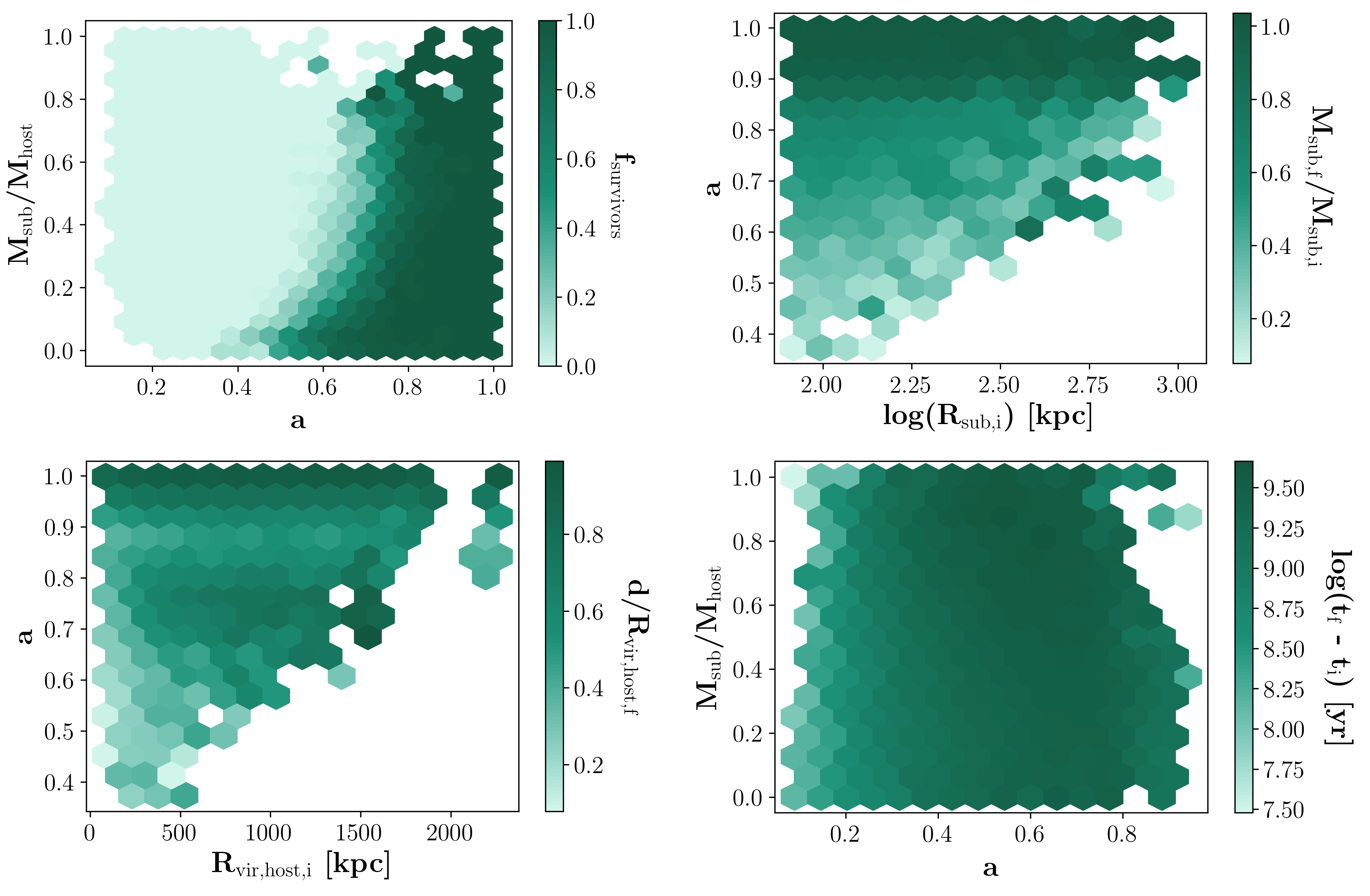
\includegraphics[width=\textwidth]{Figures/bestSpaces}
	\vspace{-15pt}
    \caption{Distributions of the predicted quantity of interest with respect to the two parameters that are most responsible for its variations. In each panel, the parameter that causes the most variation is shown on the x-axis, and the parameter that causes the second most variation is shown on the y-axis. In addition, in each panel the colorbar shows the average values of the quantity of interest within a bin. The top left panel shows the fraction of surviving subhalos. The top right panel shows the fraction of subhalo mass that remains for surviving subhalos. The bottom left panel shows the fractional distance of surviving subhalos from their host's center. The bottom right panel shows the elapsed time for a subhalo to merge. In each instance, some pattern of color striation can be seen to represent the importance of the two parameters shown. However, it is clear that the survival of a subhalo is by far the most drastically divided and well-defined by this two-dimensional space. }
    \label{fig:bestSpaces}
\end{figure*}


The advantage of using a gradient boosting regressor is again the reduction of overfitting. Because gradient boosting regressors are ensembles of weak learners, which are easier to overfit, the overall ensemble is less prone to overfitting. This is particularly important given the smaller scope of our regression problem, which uses relatively few parameters for the number of examples in our sample. As with the random forest classifier, this gradient boosting regressor class in python also contains a function to report relative feature importances. However, interpreting these results again presents difficulties due to strong correlations between parameters.

For each of our regression problems, we use a gradient boosting regressor to predict the final quantity. A different gradient boosting regression model is created and separately tuned for each of our outcomes we predict. Each model is is given all initial features to train on. As with the survival classification problem, due to the difficulty of interpreting the reported feature importances of the algorithm, we use our custom algorithm to determine the order and relative importance of features for predicting each of our desired quantities. \edits{Summary of all hypers again and what we do to tune them.}

\subsection{Other Models}
\label{sec:other models} % used for referring to this section from elsewhere
\edits{Not sure if this really needs to be its own subsection at all, or if casually mentioning this type of stuff in the previous sections is sufficient. I don't have too much to say in this section as of now but I guess it can just be a small section?}
Although we have chosen to use a random forest classifier and gradient boosting regression for our analysis, several other popular machine learning models could be chosen. In particular, neural networks have become increasingly popular for a wide variety of applications, to both classification and regression problems due to their ability to fit to data incredibly well. Several other, arguably more intuitive machine learning algorithms could also be used. The K-nearest-neighbors algorithm, for example, assigns predictions based on the properties of objects that are similar to the object trying to be predicted. To ensure that our model was as well fit and possible without being too overfit, we tried several of such machine learning algorithms before settling on our choices.

In particular, neural networks, random forests, and gradient boosting regressors seem to perform quite similarly. \edits{How much it improved/didn't improve? Specific cases? How much to say here? Reason we went with GBR's for all regressors and an RF for the survival problem? Yes to all, and OK to mention that we try and they do the same so we select the simplest ones.}

\section{Feature Selection}
\label{sec:feature selection} % used for referring to this section from elsewhere
To train our models, we have selected \textbf{INSERT NUMBER} initial parameters (or features) to describe each subhalo/host halo interaction. These parameters are selected to encompass information about the orbit, environment, and individual properties of both the host and subhalo. Although we begin with a large set of parameters for thoroughness, we expect that not all parameters will be important for predicting our desired quantities. In order to determine which parameters most strongly affect the predicted quantities, we use a feature selection method on all of the parameters that selects four parameters for each predicted quantity that are responsible for the most variation in that quantity. Because our set of parameters has strong correlations between several values, we also aim to use a feature selection method that will minimize correlations in the selected subset of features.
Although we call the methods described below "feature selection", we emphasize that we do not remove any parameters using these methods. Instead, we will use the order of selected features to determine the order in which we will add features to our models and for display purposes in our figures. During training, all models will still be given all of our parameters, to ensure that no information is missed.

\edits{I feel like this description is really inconcise and doesn't make any sense. Cant figure out a better way to word it though.} To select the subset of features, we begin by binning a predicted quantity by each of the feature parameters. Then, the most important feature parameter is the one with the most variation in average value of the predicted quantity within those bins. We define this variation as ... The next most important parameter is selected by again binning within each parameter, within the existing bins of the firstly selected parameter. We repeat this process until four feature parameters have been selected, at which point bins become to small and noisy to continue binning the data any further. The order of feature importance for each final quantity is then the order in which the parameters were selected using this method.
\aab{I agree it's hard to explain this clearly. How about this: We describe the feature selection method using the example case where we wish to predict the final mass of surviving subhalos. We begin by measuring the mean relation between the final mass and each input feature. For example, in the case of orbital eccentricity, we do this by computing the mean final mass in bins of eccentricity. We then calculate the difference between the lowest and highest values of mean final mass among the bins, as a measure of the strength of the correlation between final mass and eccentricity. We designate the feature that displays the largest such difference as the most important feature. In the next step, we create bins of this feature and we repeat the above procedure for the remaining features within these bins. In other words, we calculate the degree of correlation between final mass and each remaining feature while controlling for the most important feature. This results in a selection of the second most important feature. We continue with this process until four features have been selected, at which point the sample size does not permit further binning of the data in five dimensions. The order of feature importance for each final quantity is then the order in which the parameters were selected using this method.
}

We find this method useful for two main reasons. First, due to the strong correlations between several of our parameters, it is difficult to interpret feature importance results from the \texttt{scikit-learn} algorithms. This is because the \texttt{scikit-learn} random forest and gradient boosting regressor algorithms calculate feature importance as the information provided by a node, weighted by the fraction of total samples that pass through that node, averaged over all decision trees. This means that two parameters that contain near identical information may have similar importance rankings, despite only one being needed to make accurate predictions, \edits{as they take turns being seeded highly in different trees, after which the other one isn't needed anymore}. This can also decrease the overall importance ranking of both parameters, because \edits{it will make the same parameter be found highly important in some trees, and not important at all in others.} We found that ordering parameters according to the \texttt{scikit-learn} functionality did not lead tot he quickest information gain when training models with additional parameters. Additionally, because random forests and gradient boosting regressors are built using series of decision trees, the intuition behind those algorithms and these feature selection methods are similar. When building decision trees, features that are ranked higher in the tree are both the most important features, and those that cause the most variance in the final quantity. So, ordering our parameters by the amount of variance they are responsible, while binning to remove correlations with other parameters, leads to a feature order that appears to add information the most quickly.

The results of the four most important features for each of the predicted quantities are shown in Table \ref{tab:FS_table}. The number next to each parameter represents the strength of variance due to that feature. This number is \edits{IS... again, depends on exactly how we want to define the variance} (the normalized maximum variance within bins of that parameter? what I did here). Some parameters, such as the initial scale factor of entry and the eccentricity of the subhalos orbit, appear as important for all of the predicted quantities. In particular, the initial scale is either the first or second most important parameter for all quantities. \edits{Are these things that we would expect to physically be important/why}.

\edits{Some discussion of whether or not you can tell at this point that some thing being predicted might need an additional parameter (a fifth) or might do well with only 3 (still high variation compared to noise in the last parameter or last chosen parameter close to noise)? By looking at the numbers that are representative of the variance, which again will depend on how we define it.} Using this ranking of most important features, we look at the values of our predicted quantities within the two-dimensional space of the two parameters most responsible for variations in the outcome. This is shown in Figure \ref{fig:bestSpaces}. \edits{This figure shows... For example, the top left panel shows the mean survival fraction, in bins of both initial scale and subhalo to host halo mass ratio.} From this figure, we can see how strongly the predicted quantities rely on their chosen features. For survival, the two-dimensional space is clearly divided, suggesting that the survival of a subhalo is already well-determined by only two parameters. For the other quantities, this gradient is less defined, suggesting that either more parameters are needed to make good predictions, or the process is stochastic enough that general trends with respect to our input parameters are harder to find. In particular, the panel for merge time (lower right) in Figure \ref{fig:combined_distributions_logBin} shows little variation in outcome across the entire space of initial scale and subhalo to host halo mass ratio, despite the merging time having the strongest trend of variation with those parameters. From these two-dimensional spaces, we can already see that some of these final quantities, such as survival, may be much more straightforward to predict than others, such as merge time.

% Feature Selection Table
\begin{table}
	\centering
	\caption{The ranking order of most important features for predicting each of the desired quantities. Values next to the chosen feature represent the normalized maximum variation from binning within that parameter, where higher values indicate the parameter is more strongly responsible for changes in the prediction outcome.}
	\label{tab:FS_table}
	\begin{tabular}{c|cccc} % four columns, alignment for each
		\hline
		rank & Survival & Mass Loss & Final Position & Merge Time\\
		\hline
		1 & a () & R\textsubscript{vir,sub} () & R\textsubscript{vir,host} () & a ()\\
		2 & M\textsubscript{sub}/M\textsubscript{host} () & a () & a () & \textepsilon ()\\
		3 & \textepsilon () & \textepsilon () & M\textsubscript{sub}/M\textsubscript{host} () & M\textsubscript{sub}/M\textsubscript{host} ()\\
		4 & v\textsubscript{rel} () & d\textsubscript{rel} & \textepsilon () & c\textsubscript{sub}\\
		\hline
	\end{tabular}
\end{table}


\section{Results}
\label{sec:Results}
For each of the final quantities, we train a machine learning algorithm, using all available parameters, to predict the outcome value. For each of quantity, we select hyperparameters for the model by repeatedly training iterations of the model using the training set, and checking its accuracy on the validation set, until the best fit with lowest overfitting is achieved. For example, we may train a model with a depth hyperparameter of 5, then check if either raising the depth to 6 or lowering it to 4 with other hyperparameters held constant will give us improvement. We repeat this process for all hyperparameters, until we find a model that achieves high accuracy on both the training and validation sets, indicating that the model is well fit to the data, but with the smallest differences between training and validation accuracy, indicating that the model is minimally overfit.

Once we have found a set of hyperparameters that performs well without overfitting, we fix this as our model for the given final quantity. Then, we train this model using increasing subsets of our feature parameters and test its performance on our testing set. We begin by adding the four most important parameters, in order of their found importance, from our feature selection methods. Additional feature parameters are then randomly added, until the model is trained with all of our parameters. This gives us an accuracy for our model given not only our complete set of features, but smaller subsets of our features that utilize only the features we found to be important. In this way, we can determine the minimum subset of parameters needed to achieve maximum accuracy. 

In the following subsections, we detail the results of these models, as well as our metrics for determining the accuracy of our predictions in the case of each predicted final quantity. In Section~\ref{sec:survival}, this is discussed in detail for predicting the survival quantity. In Section~\ref{sec:mass loss}, we discuss this in detail for the mass loss quantity. In Section~\ref{sec:position} we discuss the final position quantity, and in Section~\ref{sec:merge time} we discuss the merging time quantity.

\subsection{Survival}
\label{sec:survival} % used for referring to this section from elsewhere

\begin{figure}
	% To include a figure from a file named example.*
	% Allowable file formats are eps or ps if compiling using latex
	% or pdf, png, jpg if compiling using pdflatex
	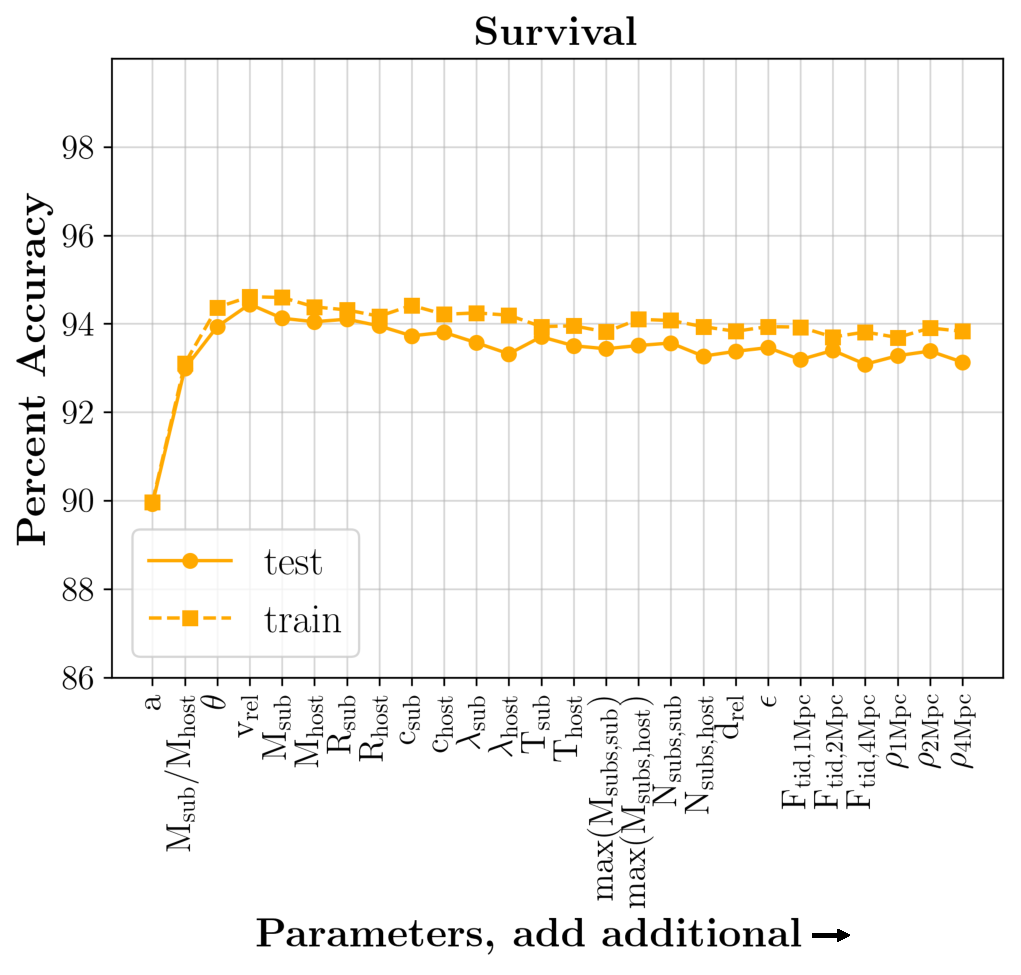
\includegraphics[width=\columnwidth]{Figures/survival_predictions}
	\vspace{-15pt}
    \caption{Accuracy of model's predictions, for both the training and testing sets, when predicting survival. Percentage of the subhalo sample that is predicted accurately is shown on the y-axis. On the x-axis, the parameters used to train the model are shown. For each point, the model was trained using all parameters to the left of that point on the y-axis. The solid line shows the accuracy on the test set, while the dashed line shows the accuracy on the set the model was trained on.}
    \label{fig:survival_predictions}
\end{figure}

\begin{figure*}
	% To include a figure from a file named example.*
	% Allowable file formats are eps or ps if compiling using latex
	% or pdf, png, jpg if compiling using pdflatex
	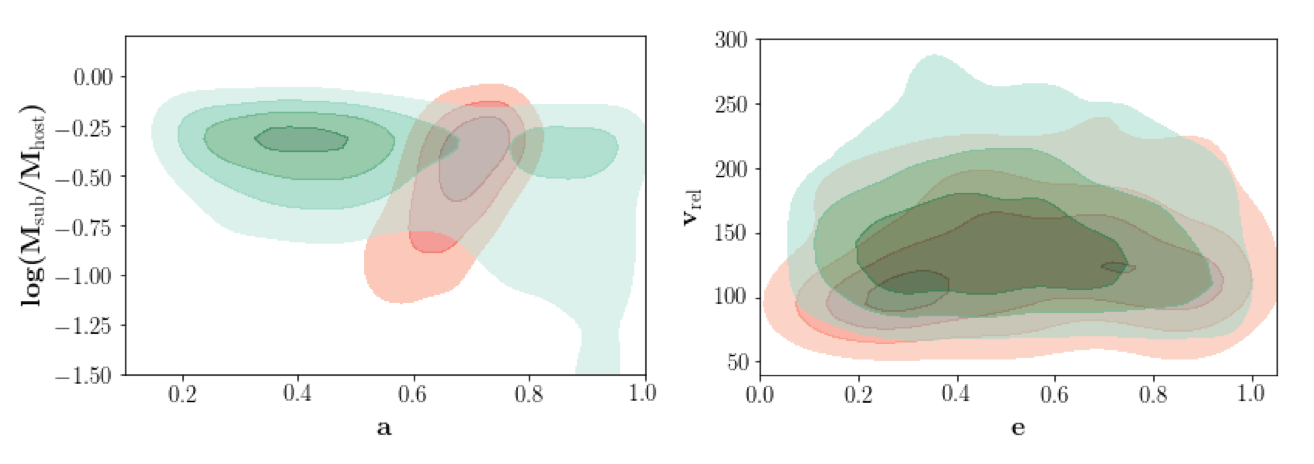
\includegraphics[width=\textwidth]{Figures/survival_contours}
	\vspace{-20pt}
    \caption{Contours of the accurately and inaccurately predicted subhalos, in two-dimensional spaces of the four most important features. Blue contours show the correctly predicted subhalos, and red contours show the incorrectly predicted subhalos. Contours are divided into 5 sections, with 20\% of subhalos lying within the inner most contour, 40\% lying within the second innermost contour, and so on. The outermost contour is not shaded as to more clearly show the contour regions.}
    \label{fig:survival_contours}
\end{figure*}

For the entire sample of subhaloes, we first try to predict whether or not a halo will survive until z=0 (assigned a value of 1) or merge with the host sometime before z=0 (assigned a value of 0) by using a random forest classifier. We tune the hyperparameters of this model and find the best results given 50 estimators and a \textit{maximum depth} of 7. We keep the \textit{max\_leaf\_nodes} hyperparameter set to the default (\texttt{None}), allowing an unlimited number of nodes at each depth. The accuracy metric we use to determine the performance of this model is a straightforward categorical accuracy, which is given as the percentage of halos correctly classified as either 0 or 1.

Figure \ref{fig:survival_predictions} shows the accuracy of this model, when trained using increasingly large subsets of our feature parameters. In this figure, each point shows the training or testing accuracy of a model trained with all parameters up to that point on the x-axis. We emphasize that, although we add parameters to the model in an ordered way, the \texttt{scikit-learn} random forest does not use the ordering of input parameters when training a model, and each new subset of parameters requires re-training of the model with that subset. Thus, if the ordering of our parameter additions had been completely random rather than chosen from our feature selection methods, the maximum model accuracy would not change, although the appearance of information gain in Figure \ref{fig:survival_predictions} would. 

As is clearly shown in Figure \ref{fig:survival_predictions}, after the addition of our three most important parameters, the accuracy of both the testing and training sets plateau, reaching a maximum of \textbf{INSERT NUMBER}\% at any point for the training set, and \textbf{INSERT NUMBER}\% at any point for the testing set. For the model trained with only these first three parameters, the testing set has an accuracy of \textbf{INSERT NUMBER}\% and the training set has an accuracy of \textbf{INSERT NUMBER}\%. The gap between these accuracies is small, suggesting low overfitting, and accuracy at this point is similar to the maximum accuracy the model reaches, suggesting a lack of significant information gained by adding any parameter thereafter. Adding further parameters causes increases or decreases in the accuracy that are within noise. Because the model is free at any iteration to use as many of the provided parameters as needed, this suggests that only these three parameters are necessary to predict the survival of a subhalo. Although the training set generally does better than the test set, the accuracy difference is small and expected due to a small amount of overfitting.

The three parameters that are needed to achieve this maximum accuracy are: the initial scale of subhalo entry, the ratio of subhalo to host halo mass, and the inclination of the subhalo orbit. With the addition of each of these parameters, a \textbf{INSERT NUMBER}, \textbf{INSERT NUMBER}, and  \textbf{INSERT NUMBER} accuracy percentage is gained for each parameter added, respectively. Within the parameter spaces of the four top parameters, we show in Figure \ref{fig:survival_contours} where the accurately and inaccurately predicted subhalos lie. There is a clear tendency for subhalos with a\textsubscript{i} =  .6 - .7 to be the most difficult to predict. This agrees with the upper left plot of Figure \ref{fig:bestSpaces}, where a clear division between always surviving and always merging occurs at this value. We note that, although most of the poorly predicted halos exist in this small section of parameter space, \textbf{INSERT NUMBER} percent of halos with a\textsubscript{i} =  .6 - .7 are still accurately predicted, significantly better than random guessing. The right panel of Figure \ref{fig:survival_contours} also shows that the innermost contour of the inaccurately predicted subhalos centers around $\epsilon$ = .4, while the innermost contour of the accurately predicted subhalos centers around $\epsilon$ = .8. Although the location of these innermost contours are clearly separated, the total span of eccentricity values is roughly the same. Similarly, the span of values for the subhalo-to-host-halo mass ratio and initial relative velocity are not noticeably different for the two populations.

\subsection{Mass Loss}
\label{sec:mass loss}
For only subhalos that survive until z=0 without being disrupted, we predict the mass of the subhalo at z=0 using a gradient boosting regressor. We tune the hyperparameters of this model and find the best results given 70 estimators, a learning rate of .05, and a \textit{max\_depth} of 10. We keep the \textit{max\_leaf\_nodes} hyperparameter set to the default (None), allowing an unlimited number of nodes at each depth. To determine the accuracy of the model, we define an accuracy metric, using the the difference between true and predicted fractional remaining mass. A subhalo is considered to be accurately predicted if:
\begin{equation}
    \label{eq:mass loss}
    \frac{|M_\textsubscript{pred,f} - M_\textsubscript{true,f}|}{M_\textsubscript{true,i}} - \frac{2m\textsubscript{p}\sqrt{N\textsubscript{p,true,i}}}{M_\textsubscript{true,i}} \leq tol
\end{equation}
Where \textit{tol} is some tolerance value which determines what difference in fractional mass loss is acceptable as accurate. We refer to the quantity given on the left hand side of the equation as the accuracy score for a given subhalo. We then vary the tolerance which we compare this score to, determining what percentage of subhalos are within certain tolerance thresholds. 

The first term in this equation is our primary measurement of the difference between our true and predicted masses. Although the quantity that our machine learning model predicts is the mass of the subhalo, we check accuracy by normalizing this value to the initial mass of the subhalo and comparing true and predicted fractions of initial mass. We do this as to have a metric that equally penalizes errors in prediction for all subhalos, rather than allowing more leniency depending on the subhalo mass. The second term in the equation acts as an additional tolerance to account for poisson noise in the number of particles assigned to the subhalo, which even a perfect predictor of the underlying mass loss process would not reasonably have errors less than. This term is significantly smaller than the first term and only makes a difference in the case of small subhalos, where a small number of particles is a larger portion of the mass than in larger subhalos.

Figure \ref{fig:massloss_predictions} shows the accuracy of best-fit model, when trained using all and increasingly small subsets of the feature parameters. Because accuracy of this model depends on the selected tolerance value, we show the accuracy given several different choices of tolerance. Again, the training set generally does better than the test set, for all tolerances, due to slight  overfitting. It can be seen that, again using only the three top-ranking parameters, 60\% of subhalos have their final masses accurately predicted to with a margin of error of less than \textpm 5\% of their true initial mass. 90\% of subhalos can be predicted accurately, given predictions within \textpm 20\% of their initial mass. Almost all subhalos can have their masses predicted to within \textpm 50\% of their initial mass, although it's worth noting that, in the instance of a subhalo that loses half of its mass, that would allow the full range of losing none to all of its mass to be considered accurate. 

Although a significant fraction of our subhalo population cannot have their final masses predicted with high precision, we point out that this model still performs much better than a naive guess. As a baseline model, we assign a predicted final mass fraction to all subhalos as the average final mass fraction of the sample. Using Equation \ref{eq:mass loss} to calculate the accuracy of this baseline model, we find that only 15\% of subhalos have their final masses accurately predicted to with a margin of error of less than \textpm 5\% of their true initial mass, 65\% with a margin of error less than \textpm 20\% of their true initial mass, and 93\% with a margin of error less than \textpm 50\% of their true initial mass. It is clear that, although the majority of subhalos can be predicted to within \textpm 50\% of their true initial mass by both models, our machine learning model has much improvement over the baseline model for making more precise predictions.

The three parameters needed before prediction accuracy levels off with the addition of more parameters are: the radius of the subhalo, the initial scale factor, and the subhalo's orbital inclination. Again, given the ordering from the feature selection methods discussed above, these parameters show the quickest gain of information with the quickest leveling off of additional accuracy, even given a model allowed to select any of the full 26 parameter set. Adding these first three parameters results in an increase of \textbf{INSERT NUMBER}, \textbf{INSERT NUMBER}, and  \textbf{INSERT NUMBER} accuracy percentage gain, respectively. 

Within the parameter spaces of the four top parameters, we show in Figure \ref{fig:massloss_contours} where the subhalos with the best and worst 10\% of accuracy scores lie. Most of the best-predicted subhalos are those that enter their host closer to z=0, with the contours centering around a\textsubscript{i} = .95, likely because those do not have much time to lose mass before the end of the simulation, and thus have final masses similar to their initial masses. Larger subhalos, given by larger radii, also appear more difficult to predict than their smaller counterparts, with the span of radii for the best predicted subhalos being both centered around smaller radii and not spanning to large radii. As the radius of a subhalo is analog to its mass, this also means that less massive subhalos are easier to predict than their more massive counterparts. The best predicted subhalos also seem to have higher eccentricities than their poorly predicted counterparts, although the span of eccentricities is the same for both. The span of initial relative distances is different for the best and worst predicted populations, with the best predicted subhalos spanning across a larger range of relative distances, despite the centers of the contours being roughly the same.

\begin{figure}
	% To include a figure from a file named example.*
	% Allowable file formats are eps or ps if compiling using latex
	% or pdf, png, jpg if compiling using pdflatex
	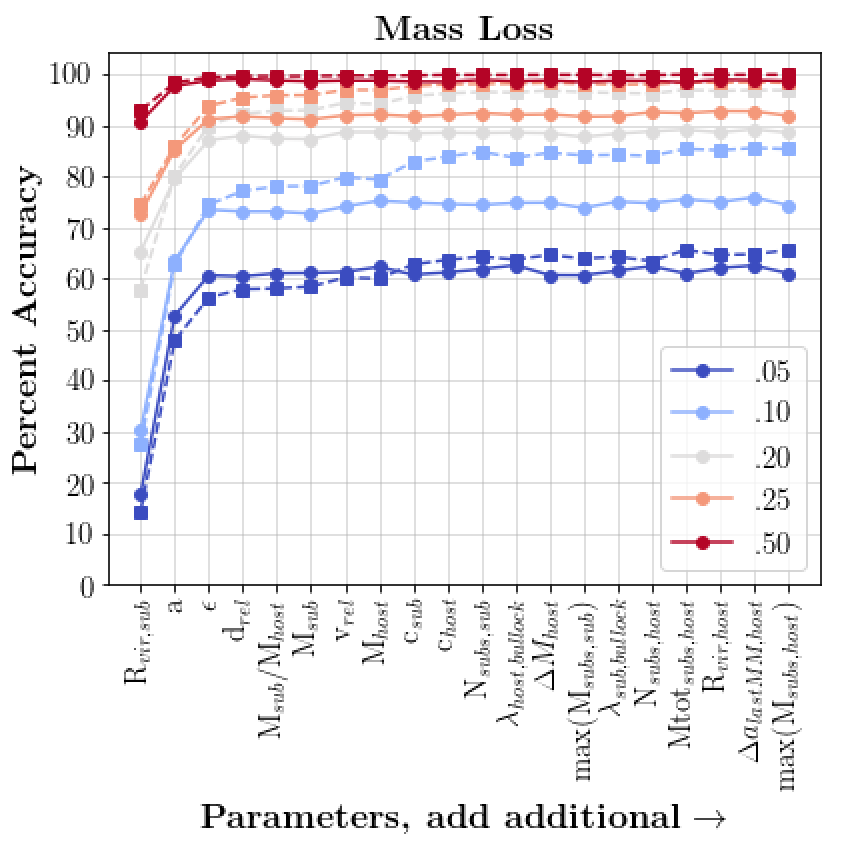
\includegraphics[width=\columnwidth]{Figures/massloss_predictions}
	\vspace{-15pt}
    \caption{Accuracy of model's predictions, for both the training and testing sets, when predicting mass loss. Percentage of accurate predictions is shown on the y-axis. The x-axis shows parameters used to train the model. For each point, the model was trained using all parameters to the left of that point on the y-axis. The solid line shows the accuracy on the test set, while the dashed line shows the accuracy on the set the model was trained on. Different colored lines show the different tolerance values used to define accuracy, as defined in Equation \ref{eq:mass loss}. For a complete description of this accuracy metric, see text.}
    \label{fig:massloss_predictions}
\end{figure}

\begin{figure*}
	% To include a figure from a file named example.*
	% Allowable file formats are eps or ps if compiling using latex
	% or pdf, png, jpg if compiling using pdflatex
	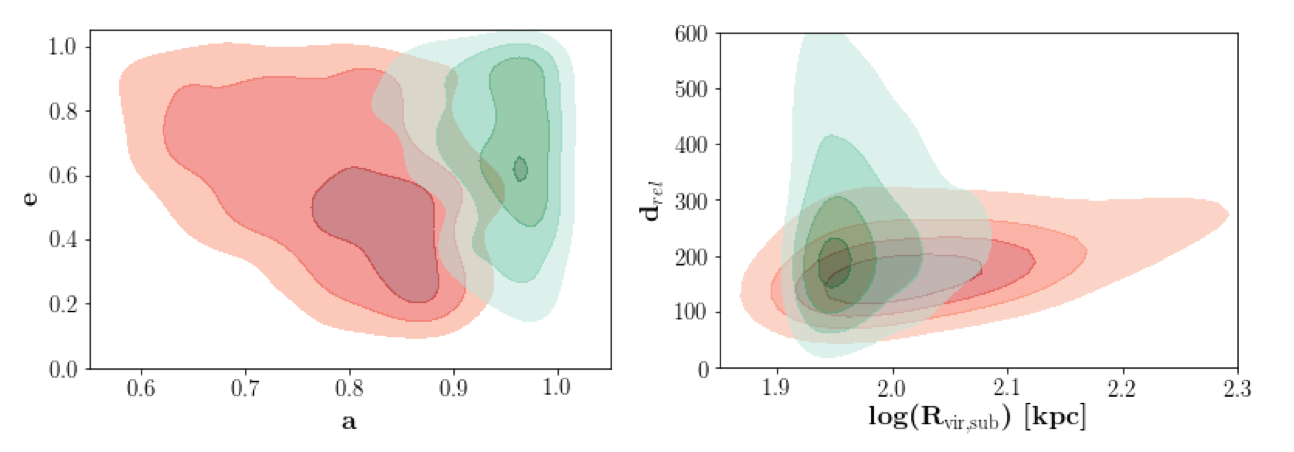
\includegraphics[width=\textwidth]{Figures/massloss_contours}
	\vspace{-20pt}
    \caption{Contours of the top and bottom 25\% accuracies of predicted subhalos, in the two-dimensional spaces of the four most important features. Blue contours show the best predicted subhalos, and red contours show the worst predicted subhalos. Contours are divided into 5 sections, with 20\% of subhalos lying within the inner most contour, 40\% lying within the second innermost contour, and so on. The outermost contour is not shaded as to more clearly show the contour regions.}
    \label{fig:massloss_contours}
\end{figure*}

\subsection{Final Position}
\label{sec:position}
For only subhalos that survive until z=0 without being disrupted, we next predict the final position of the subhalo at z=0, relative to the center of the host halo, using a gradient boosting regressor. We tune the hyperparameters of this model and find the best results given 50 estimators, a learning rate of .05, and a \textit{max\_depth} of 10. We keep the \textit{max\_leaf\_nodes} hyperparameter set to the default (None), allowing an unlimited number of nodes at each depth. To determine the accuracy of the model, we define an accuracy metric, using the the difference between true and predicted fractional distance from host center. A subhalo is considered to be accurately predicted if:
\begin{equation}
    \label{eq:position}
    |d_\textsubscript{rel,f,true} - d_\textsubscript{rel,f,pred}| - \frac{2R\textsubscript{soft}}{R_\textsubscript{host,f}} \leq tol
\end{equation}
Where \textit{tol} is some tolerance value which determines what difference in fractional distance from host center is acceptable as accurate. As when predicting the mass loss quantity, the left hand side of this equation determines the accuracy score, and we vary the tolerance to set different thresholds for what accuracy score we will consider as an accurate prediction. The first term in this equation is simply the absolute difference between the true and predicted fractional distance from host center. Because what our model predicts is the actual fractional distance of the subhalo from the host halo center, we do not need to additionally normalize this quantity as we did when predicting mass loss, as this value can be straightforwardly taken as the fraction of the host radius by which the prediction is off. The second term in the equation is an additional tolerance, to account for uncertainty in the subhalo's position within its host due to the softening length.

Figure \ref{fig:position_predictions} shows the accuracy of best-fit model, when trained using all and increasingly small subsets of the feature parameters. Because accuracy of this model depends on the selected tolerance value, we show the accuracy given several different choices of tolerance. Again, the training set generally does better than the test set, for all tolerances, due to slight  overfitting. For final position, it appears that more parameters are needed to reach maximum accuracy, with the first five given parameters being used for predictions before accuracy levels off. For final position, predictions are slightly worse than for mass loss. 50\% of subhalos can be predicted to \textpm 5\% of their true fractional distance. 90\% of subhalos can be predicted accurately, given their prediction requires accuracy to only \textpm 20\% of their true fractional distance. Almost all subhalos can have their final position predicted to within \textpm 50\% of their final fractional mass. As with mass loss, we note that a tolerance of .5 is very lenient, allowing the full range of the subhalo lying anywhere within the host as an accurate prediction.

\edits{Comparing these prediction accuracies to a baseline model again 

The five parameters needed before prediction accuracy levels off with the addition of more parameters are: the radius of the host halo, the initial scale factor, the mass ratio between the sub and host halo, the subhalo's orbital inclination, and the relative velocity with which the subhalo enters. Given the ordering from the feature selection methods discussed above, it appears that these parameters were chosen to be quite important, although the mass ratio provides less accuracy gain than some of the other, later-chosen parameters. Adding these first five parameters results in an increase of \textbf{INSERT NUMBER}, \textbf{INSERT NUMBER}, \textbf{INSERT NUMBER}, \textbf{INSERT NUMBER}, and  \textbf{INSERT NUMBER} accuracy percentage gain, respectively. Within the parameter spaces of the four top parameters, we show in Figure \ref{fig:position_contours} where the best and worst 10\% of predicted subhalos lie. Most of the best-predicted subhalos are those that enter their host closer to z=0, likely because those have less time to move deep into the host and have their orbits altered as much. The radius of the host appears to span roughly the same space for both populations, with the worst predicted subhalos being concentrated more towards smaller host radii than their better predicted counterparts. The two-dimensional space of mass ratio and orbital inclination is nearly identical for the two populations,

\begin{figure}
	% To include a figure from a file named example.*
	% Allowable file formats are eps or ps if compiling using latex
	% or pdf, png, jpg if compiling using pdflatex
	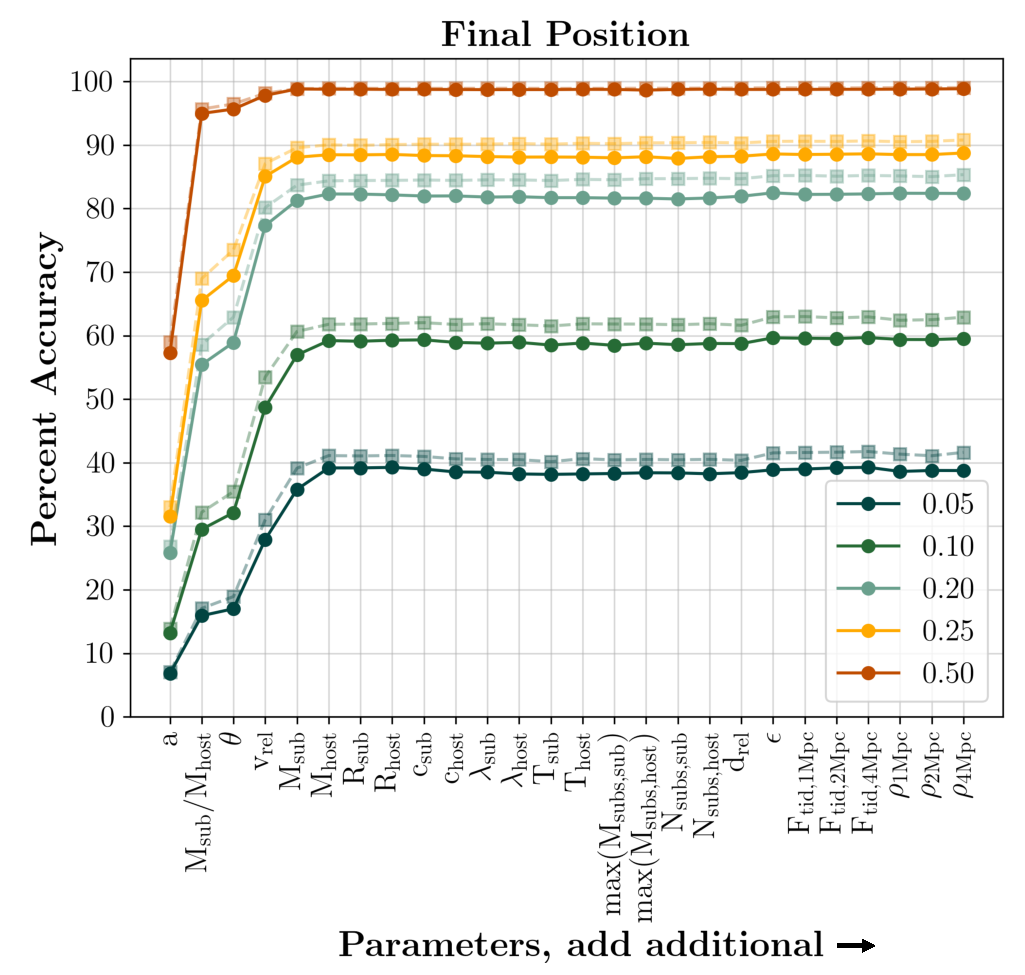
\includegraphics[width=\columnwidth]{Figures/position_predictions}
	\vspace{-15pt}
    \caption{Same as Figure \ref{fig:massloss_predictions}, but for the final position prediction. Different colored lines show the different tolerance values used to define accuracy, as defined in Equation \ref{eq:position}. For a complete description of this accuracy metric, see text.}
    \label{fig:position_predictions}
\end{figure}

\begin{figure*}
	% To include a figure from a file named example.*
	% Allowable file formats are eps or ps if compiling using latex
	% or pdf, png, jpg if compiling using pdflatex
	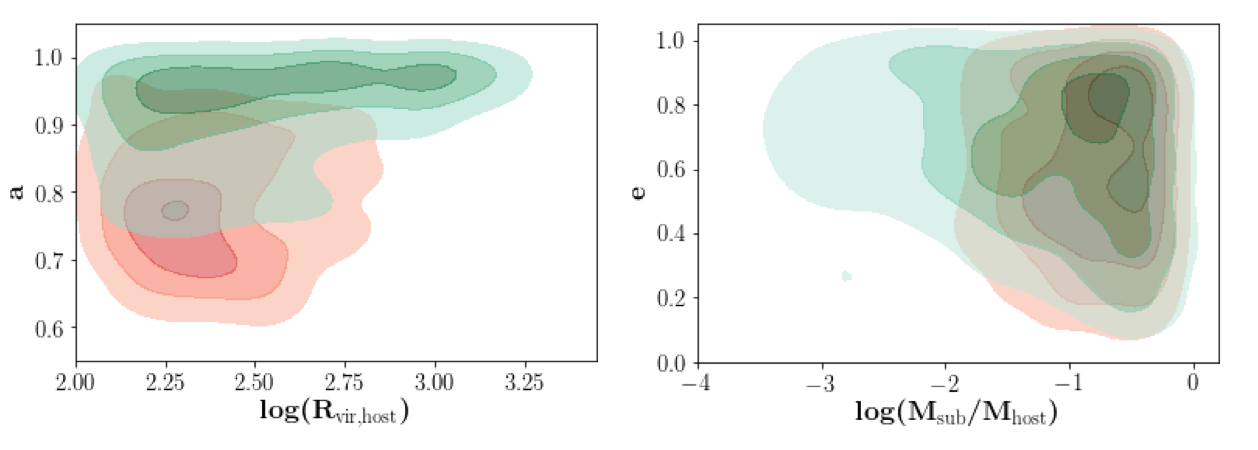
\includegraphics[width=\textwidth]{Figures/position_contours}
	\vspace{-20pt}
    \caption{Same as \ref{fig:massloss_contours}, but for the final position parameters and predictions.}
    \label{fig:position_contours}
\end{figure*}

\subsection{Merge Time}
\label{sec:merge time}
For only subhalos that have merged before z=0, we finally predict the amount of elapsed time between the subhalos entry and subsequent merging, using a gradient boosting regressor. To determine the accuracy of the model, we define an accuracy metric, using the the difference between true and predicted number of crossing times. A subhalo is considered to be accurately predicted given:
\begin{equation}
    \label{eq:time}
    \frac{|t_\textsubscript{f,true} - t_\textsubscript{f,pred}|}{t_\textsubscript{cross,f,true}} \leq tol
\end{equation}
Where \texit{tol} is some tolerance value which determines to within how many crossing times a prediction is considered to be accurate. \edits{Chosen because.}

Figure \ref{fig:time_predictions} shows the accuracy of best-fit model, when trained using all and increasingly small subsets of the feature parameters. Because accuracy of this model depends on the selected tolerance value, we show the accuracy given several different choices of tolerance. Again, the training set generally does better than the test set, for all tolerances, due to slight  overfitting. To predict merging time, again only three parameters appear to be necessary to reach maximum accuracy. 50\% of subhalos can be predicted to within half of a crossing time. 90\% of subhalos can be predicted accurately, given their prediction requires accuracy to only within 1.5 crossing times. All subhalos can have their merging time predicted to within five crossing times. Again, we emphasize that 5 crossing times is typically around 1 billion years.

The three parameters needed before prediction accuracy levels off with the addition of more parameters are: the initial scale factor, the subhalos orbital eccentricity, and the mass ratio between the sub and host halo. Adding these first three parameters results in an increase of \textbf{INSERT NUMBER}, \textbf{INSERT NUMBER}, and  \textbf{INSERT NUMBER} accuracy percentage gain, respectively. Within the parameter spaces of the four top parameters, we show in Figure \ref{fig:position_contours} where the best and worst 25\% of predicted subhalos lie. Most of the best-predicted subhalos have masses more similar to their host halos. The worst-predicted subhalos also appear to have lower concentrations than their better-predicted counterparts. \edits{Say more.}

\begin{figure}
	% To include a figure from a file named example.*
	% Allowable file formats are eps or ps if compiling using latex
	% or pdf, png, jpg if compiling using pdflatex
	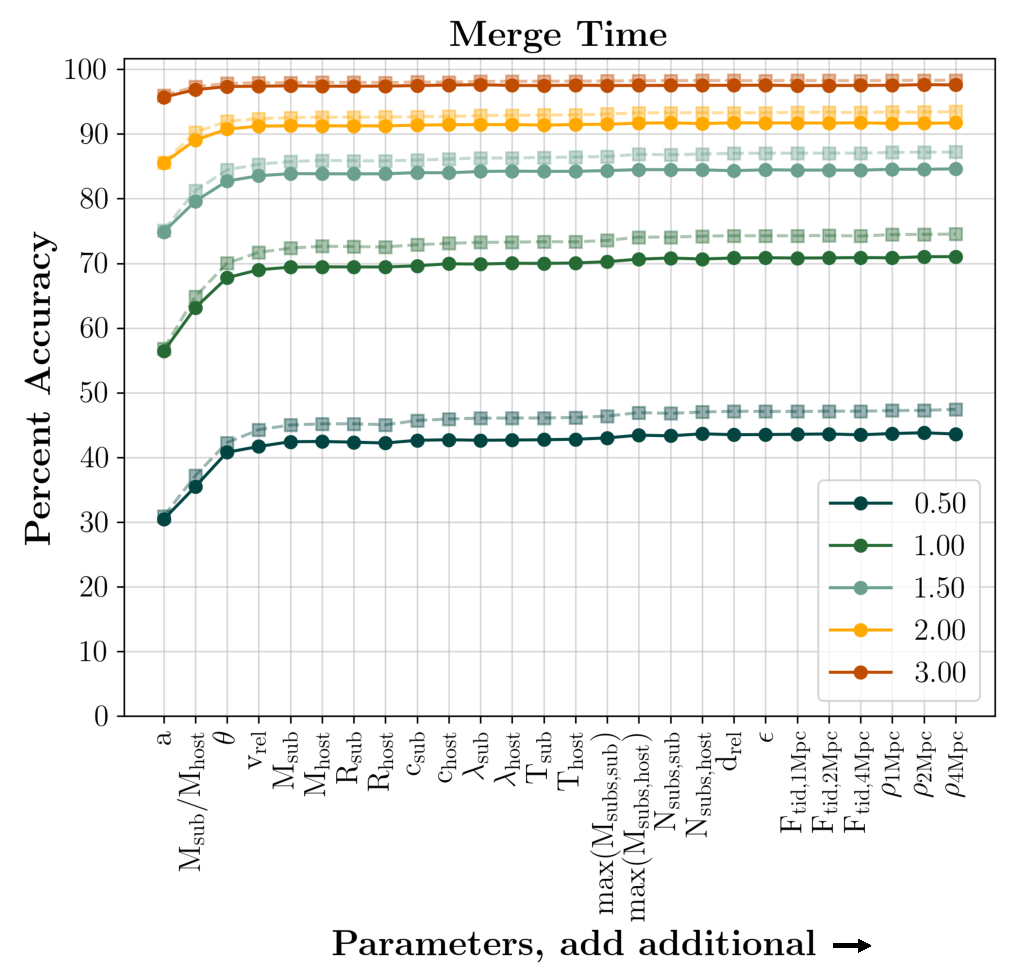
\includegraphics[width=\columnwidth]{Figures/time_predictions}
	\vspace{-15pt}
    \caption{Same as Figure \ref{fig:massloss_predictions}, but for the merge time prediction. Different colored lines show the different tolerance values used to define accuracy, as defined in Equation \ref{eq:time}. For a complete description of this accuracy metric, see text.}
    \label{fig:time_predictions}
\end{figure}

\begin{figure*}
	% To include a figure from a file named example.*
	% Allowable file formats are eps or ps if compiling using latex
	% or pdf, png, jpg if compiling using pdflatex
	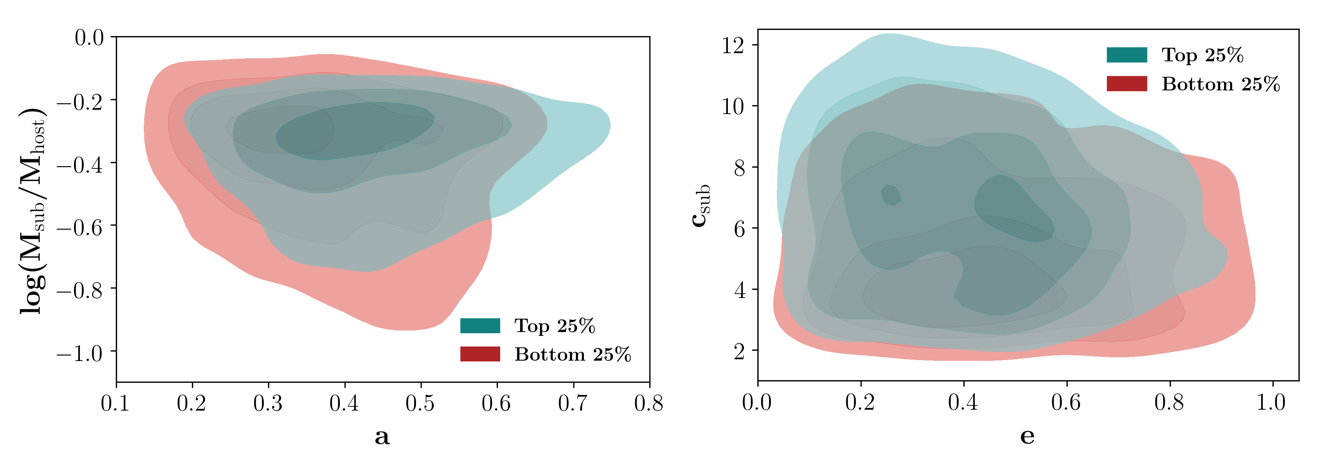
\includegraphics[width=\textwidth]{Figures/time_contours}
    \vspace{-20pt}
    \caption{Same as \ref{fig:massloss_contours}, but for the merge time parameters and predictions.}
    \label{fig:time_contours}
\end{figure*}


\section{Summary and Discussion}
\label{sec:Conclusion}
In this paper, we have used machine learning algorithms to fit a model that predicts the survivial, mass loss, final position, and merge time of a subhalo from parameters taken right at the time of its infall. Our goals were to better understand to what degree these final outcomes are due to stochasticity in subhalo evolution versus real, physically-motivated processes that could be consistently, analytically predicted. From predictions based on these models, we have found:
\begin{itemize}
    \item Subhalo survival can be predicted remarkably well, with 96.5\% of our sample being correctly predicted as surviving or disrupting. These predictions need only three initial parameters: the scale factor at the time of the start of the interaction, the mass ratio between the subhalo and its host, and the orbital eccentricity, but the initial scale factor is by far the most influential of these parameters. Subhalos with both late and early entry times are easiest to predict, while those entering their host halos at a = ~.65 are much more difficult. \edits{Is this mass dependent? True for all or a certain type? For other mass ratios is there a different turnover?}
    \item Subhalo mass loss is, a generally stochastic process. Although 60\% of our sample can be correctly predicted to \edits{within 5\% of their initial masses correct statement?}, an accuracy of 90\% is only achieved given predictions are accurate to within 20\% of their initial mass. These predictions also need only three initial parameters: the virial radius of the subhalo, the scale factor at the time of the start of the interaction, and the orbital eccentricity. Smaller subhalos with late entry times are easier to predict than their larger or earlier counterparts.
    \item Subhalo final locations are also difficult to predict. 50\% of our sample can be correctly predicted to within \textpm 5\% of their the host virial radius, but an accuracy of 90\% is only achieved given predictions are accurate to within 20\% of the host virial radius. These predictions need five initial parameters: the virial radius of the host halo, the scale factor at the time of the start of the interaction, the mass ratio between the sub and host halo, the orbital eccentricity, and the initial relative velocity.
    \item Subhalo merging timescales are also difficult to predict. 50\% of our sample can be correctly predicted to within half of their initial crossing time, but an accuracy of 90\% is only achieved given predictions are accurate to within 1.5 crossing times. These predictions again need only three parameters: the scale factor at the time of the start of the interaction, the orbital eccentricity, and the mass ratio between the sub and host halo. 
    \item There are some interesting commonalities among both the sets of parameters needed to make these predictions and the parameter spaces in which predictions are poorest. Only five parameters, in total, are needed to achieve the maximum prediction accuracy for all of our predicted outcomes. The scale factor, orbital eccentricity, relative velocity, and the masses of the host and subhalo (sometimes combined as mass ratio or appearing as virial radius instead) appear to be the only relevant parameters for determining subhalo evolution. Additionally, the parameter spaces that are most difficult to make predictions within also have much overlap. In general, subhalos that enter at a mid-range of initial scales (typically a = .6-.8) are challenging to make predictions for, across all of our final outcomes. There also appear to be trends in eccentricity, with higher eccentricities (more circular orbits) being easier to predict the behavior of, except for in the case of predicting disruption, where the opposite appears to be true.
    \item \edits{Anything else? Like is there anything common among the halos that are predicted poorly for different parameters (are the same halos or types of halos predicted poorly across multiple outcomes) that isn't in the set of params we showed in the contours? Do we want to get into that?}
\end{itemize}

It is clear from our results that, for predicting the mass loss, final location, and merging timescales of individual subhalos, an accurate, consistent mapping cannot be found given our set of initial parameters. There are several possible reasons for this inability to accurately model subhalo evolution. The first possibility is that some parameter or parameter was missing from the initial set, which would have been fundamental to making accurate predictions. Although we have made sure to include parameters that were found in the literature to be important for modeling these outcomes, our list was not completely comprehensive with all possible information. For instance, some additional parameters that we could have chosen to include are: \edits{Need to check original list we had/ depends on final set we choose in section 2}. However, as we have done an extensive search of the literature to find relevant parameters and include them in our models, we have no reason to believe that these excluded parameters would be able to contribute such a significant portion of the needed information. So, although the possibility remains that additional parameters could be needed to improve predictions, it seems unlikely that the missing information could be completely encompassed there.

A second possibility is that errors within the simulation, halo catalog, or merger tree make subhalo evolution unpredictable and sometimes incorrect. Much speculation remains as to the accuracy of these simulations, particularly on these small scales (Van den Bosch 2018, VDB 2016, everything VDB's done pretty much). Although several studies have suggested that simulation resolution only effects subhalos with fewer than 50-100 particles (CITE, CITE, CITE), \citet{VandenBosch2018} found that typical state-of-the-art cosmological simulations cannot resolve subhalos well enough to follow their mass loss until complete disruption. In the Bolshoi simulation, \citet{VDB2016} found that only around 20\% of subhalo disruption was truly physical, with instantaneous masses of the subhalos along their orbits being highly erratic. Similarly, \citet{VandenBosch2017} found that most subhalo disruption in modern simulations is artificial or numerical in nature. \edits{talk more about at what mass? what number of particles? where exactly would this hurt us.} A number of other works have also called into question the reliability of the halo catalogs and merger trees that are generated from these simulations. Comparison projects have found differing results for the fates of subhalos using different halo finders (\citet{Knebe2011}, \citet{Onions2012}, \citet{Avila2014}, \citet{Behroozi2015}) and merger tree codes (\citet{Srisawat2013}, \citet{Jiang2014}). Because these codes fundamentally define subhalos in different ways and trace their properties between snapshots using different methods, these comparison projects found that, when applied to the same simulation, resulting halo catalogs and merger trees could differ quite significantly. \edits{A few more specific examples, in each case. Need more citations/projects.}
However, although the accuracy of simulation results have been brought into question, again, we note that it seems unlikely that these errors could be entirely responsible for the results we have found. \citet{VandenBosch2018} found that, despite physical disruption being extremely rare within simulations, subhalos only became highly sensitive to numerical disruption after losing over about 90\% of their mass. Additionally, even though (CITE, CITE) found errors in the mass loss histories of subhalos within simulations using Rockstar, the overall mass losses were smooth, and since our study only relies on final outcomes mapping from the initial conditions, minor errors along the history should not be important. \edits{Are these resolution effects deterministic? i.e could they be our stochasticity or no}

Another possibility is that final outcomes can be accurately predicted from initial conditions of the interaction, but the machine learning methods used here were not able to capture the process. This could be due to a few reasons. It is possible that the particular machine learning method used was not well-suited to the problem. However, we have extensively tried different algorithms, from very simple methods to neural networks, and have found that the results given here are the best we could possibly do. Another possibility is that we did not have enough data or the data did not span the space well enough. \edits{Citations that it was enough data? Talk about how we reduced the dataset and got the same results.}

The final possibility, and the one that we believe to be the most likely explanation, is that there is an inherent non-deterministic nature of these interactions. In this case, the initial conditions of an interaction are not enough to know the outcome, because similar initial conditions can lead to very different outcomes. In \ref{fig:stdev_bestSpaces}, we show the standard deviation of outcomes within bins in two-dimensional space of the top two most important parameters for each outcome. It becomes clear in this figure that, even for very narrow ranges of parameter space, outcomes can have a wide range of values. This further suggests that an inherent stochasticity within the merging process is likely the reason predictions are so difficult to get accurately. This also agrees with the contour plots shown in Figures \ref{fig:survival_contours}, \ref{fig:massloss_contours}, \ref{fig:position_contours}, and \ref{fig:time_contours}, which show that the regions of parameter space in which the machine learning models make the worst predictions are also the spaces in which there is the widest range of outcomes for similar initial conditions.

Several papers (\textbf{CITE, CITE, CITE}) have noted that interactions between subhalos as they orbit within their hosts can be frequent and lead to significant amounts of mass loss. \textbf{CITE} found that penetrating interactions between subhalos can be the cause of nearly 40\% of a subhalos mass loss, whereas \textbf{CITE} found that the buildup of minor interactions over a subhalos life can be significant. In order to test if this is a possible cause of the stochasticity that we've found, we track the number of interactions that each of our subhalos has during its infall into its host. By counting the number of other subhalos that come within 2 virial radii of the center of each subhalo,

\edits{Possible use/implications for simulation.}An inherent stochasticity in these merging processes within has implications for simulations and the models that are built from them.  \edits{What can we say about the results of simulations or how they do their calculations of these types of merging interactions based on the uncertainty in the outcomes of the objects? How much can we expect this type of uncertainty and is it a cause for concern.
 Can you still use these models to make predictions for galaxy evolution? Assigning populations from these distributions. YES EXPAND.}

\edits{Possible use/implications for observation. Is there anything we can say about distributions that we can expect around the MW or other galaxies. Particularly for survival which we obviously predict much better than the other quantities.} Although the inability to accurately model subhalo evolution points to stochasticity in merging processes, 

In this study, we have used a dark matter only simulation for to study the evolution of subhalos. However, hydrodynamic simulations can also be used to study subhalo evolution, in the more complete context of baryonic physics as well. It remains to be seen and would be interesting to explore the implications of baryons in this type of work. Although subhalo disruption and evolution in dark matter only simulations appears stochastic and difficult to predict, hydrodynamic simulations may be differently behaved. Additionally, given that this type of works gives some insight as to what parameters are most prominent in determining how a subhalo evolves, a similar study using a hydrodyanmic simulation could confirm or oppose these findings, providing interesting insights to the differences between these types of simulations. 


\begin{figure*}
	% To include a figure from a file named example.*
	% Allowable file formats are eps or ps if compiling using latex
	% or pdf, png, jpg if compiling using pdflatex
	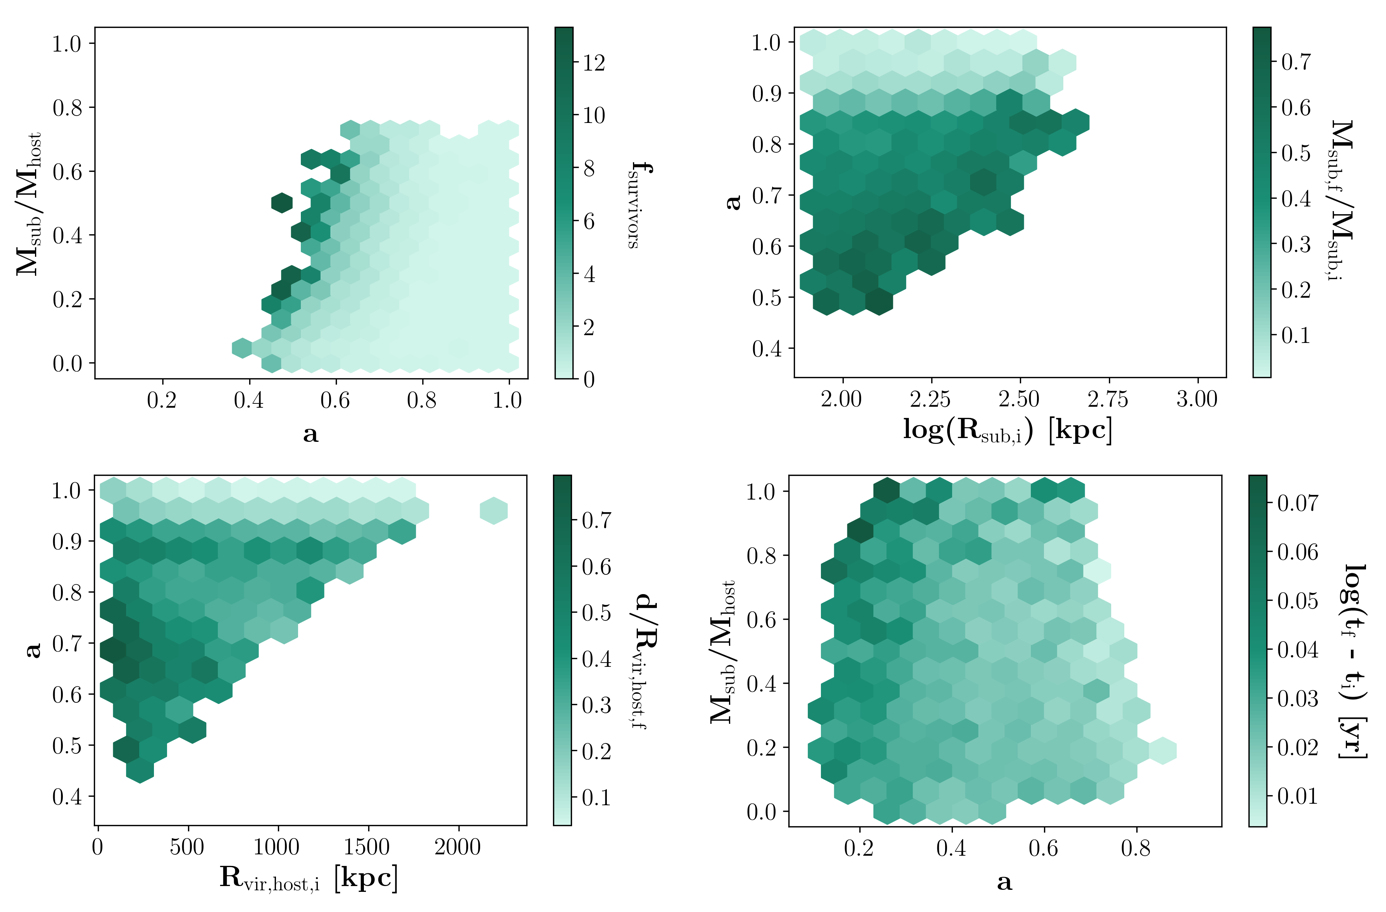
\includegraphics[width=\textwidth]{Figures/stdev_bestSpaces}
	\vspace{-20pt}
    \caption{Same as Figure \ref{fig:bestSpaces}, but each hexagonal bin contains the average standard deviation, normalized by the average value within that bin.}
    \label{fig:stdev_bestSpaces}
\end{figure*}

\section*{Acknowledgements}

I would like to thank the academy, ...

%%%%%%%%%%%%%%%%%%%%%%%%%%%%%%%%%%%%%%%%%%%%%%%%%%

%%%%%%%%%%%%%%%%%%%% REFERENCES %%%%%%%%%%%%%%%%%%

% The best way to enter references is to use BibTeX:

\bibliographystyle{mnras}
\bibliography{mendeley.bib}

%%%%%%%%%%%%%%%%%%%%%%%%%%%%%%%%%%%%%%%%%%%%%%%%%%

%%%%%%%%%%%%%%%%% APPENDICES %%%%%%%%%%%%%%%%%%%%%

\appendix

\section{Some extra material}

If I wanted to present additional material which would interrupt the flow of the main paper, that would go here.

%%%%%%%%%%%%%%%%%%%%%%%%%%%%%%%%%%%%%%%%%%%%%%%%%%


% Don't change these lines
\bsp	% typesetting comment
\label{lastpage}
\end{document}

% End of mnras_template.tex